\documentclass{standalone}
\usepackage{tikz}
\usetikzlibrary{patterns, positioning}
\usepackage[sfdefault]{ClearSans} %% option 'sfdefault' activates Clear Sans as the default text font
\usepackage[T1]{fontenc}

\begin{document}
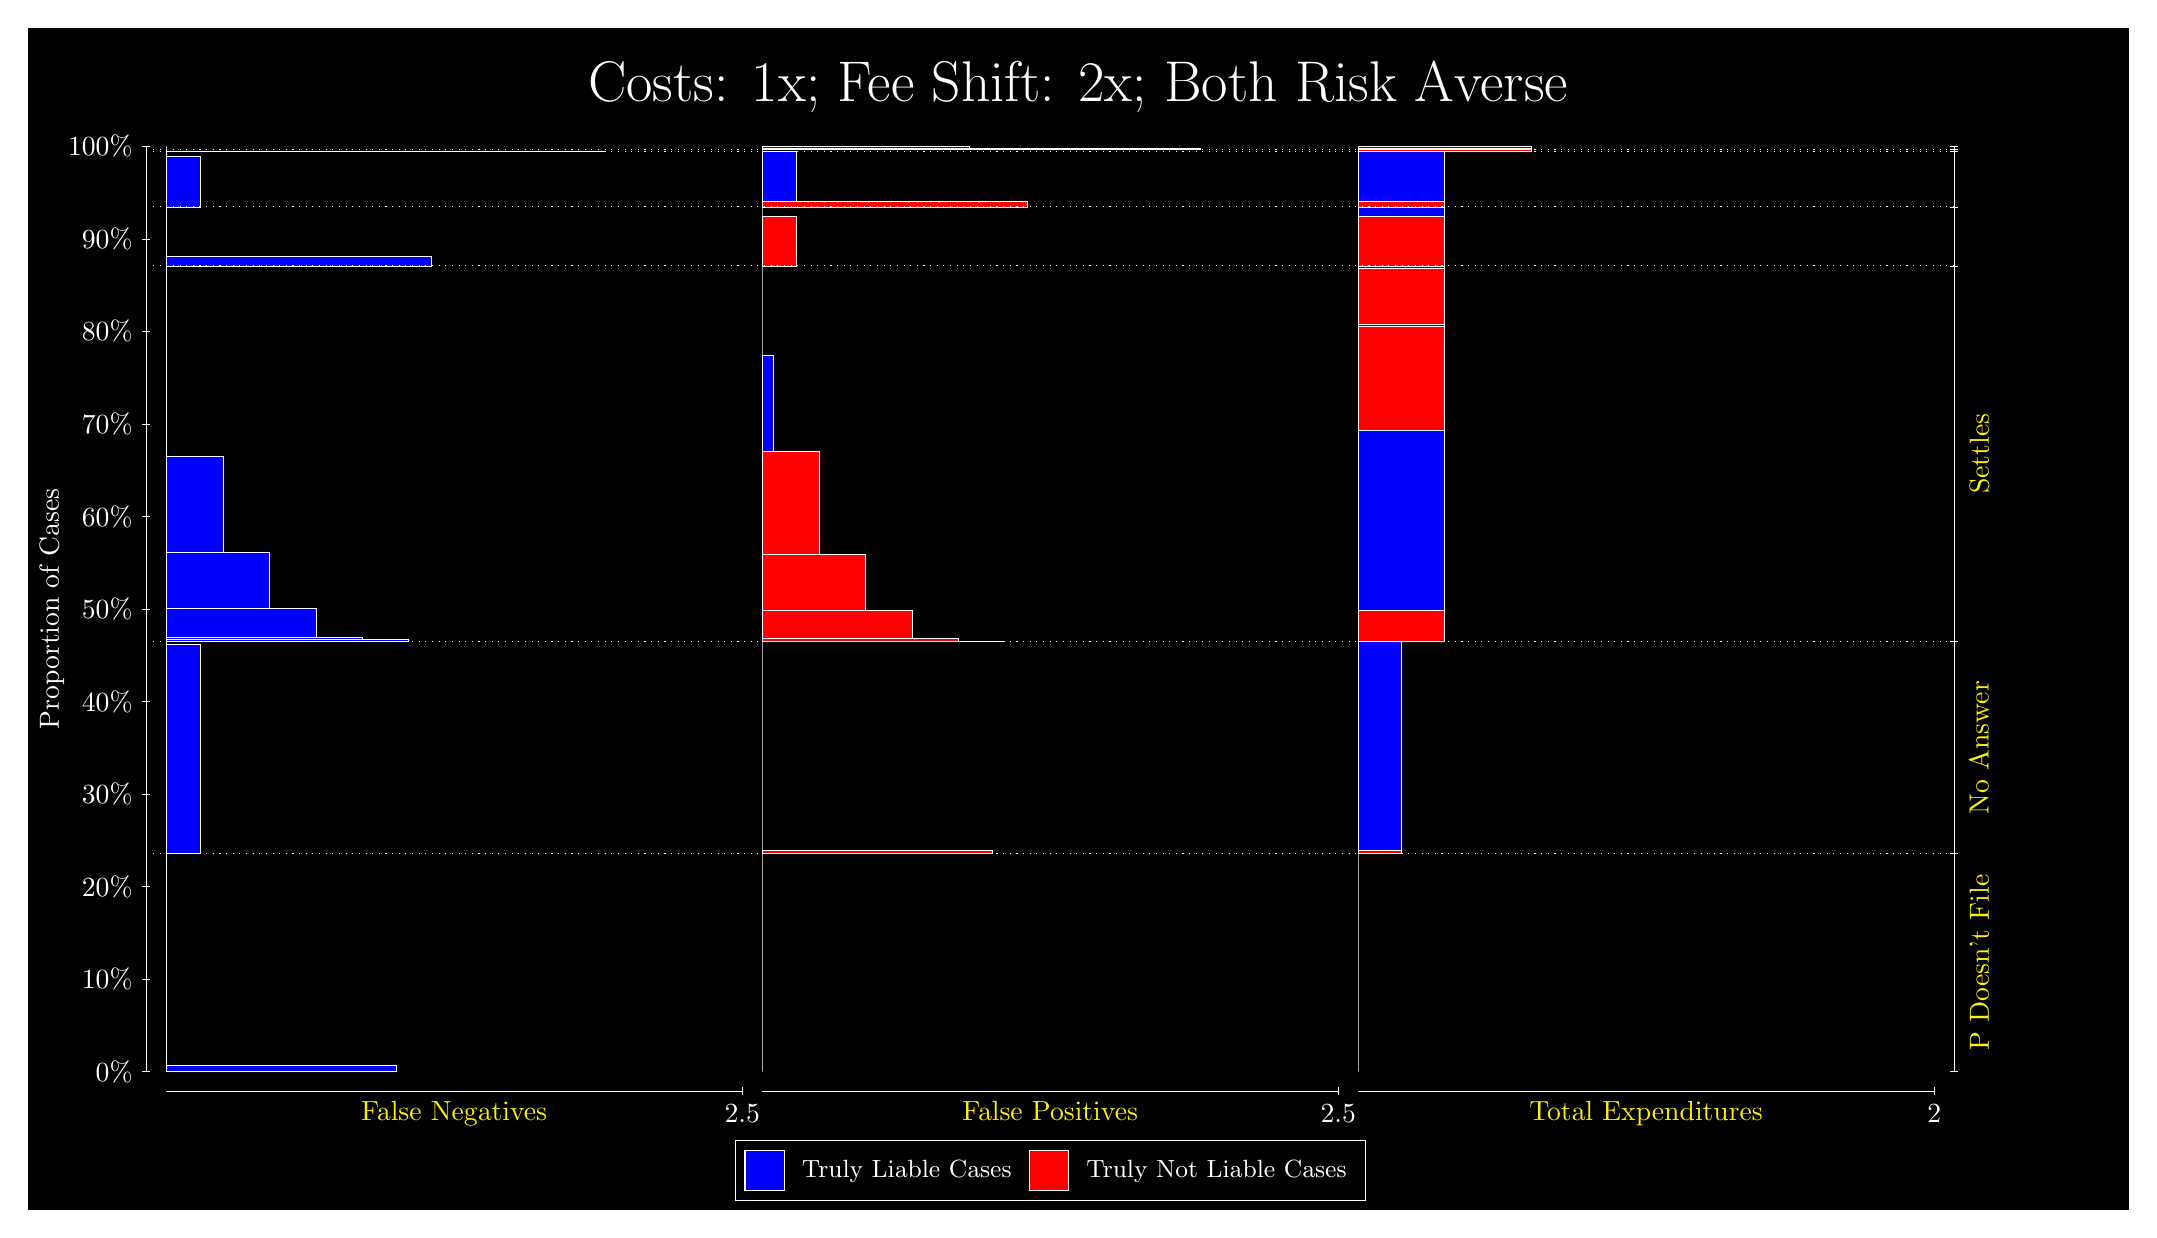
\begin{tikzpicture}
\draw[fill=black] (0,0) rectangle (26.667,15);
\draw[text=white] (0,13.5) rectangle (26.667,15) node[midway] {\huge Costs: 1x; Fee Shift: 2x; Both Risk Averse};
\draw[white, very thin] (1.5,1.75) -- (1.5,13.5);
\node[rotate=90, text=white, anchor=center] at (0.3, 7.625) {Proportion of Cases};
\draw[white, very thin] (1.45,1.75) -- (1.55,1.75);
\node[text=white, anchor=east] at (1.45, 1.75) {0\%};
\draw[white, very thin] (1.45,2.925) -- (1.55,2.925);
\node[text=white, anchor=east] at (1.45, 2.925) {10\%};
\draw[white, very thin] (1.45,4.1) -- (1.55,4.1);
\node[text=white, anchor=east] at (1.45, 4.1) {20\%};
\draw[white, very thin] (1.45,5.275) -- (1.55,5.275);
\node[text=white, anchor=east] at (1.45, 5.275) {30\%};
\draw[white, very thin] (1.45,6.45) -- (1.55,6.45);
\node[text=white, anchor=east] at (1.45, 6.45) {40\%};
\draw[white, very thin] (1.45,7.625) -- (1.55,7.625);
\node[text=white, anchor=east] at (1.45, 7.625) {50\%};
\draw[white, very thin] (1.45,8.8) -- (1.55,8.8);
\node[text=white, anchor=east] at (1.45, 8.8) {60\%};
\draw[white, very thin] (1.45,9.975) -- (1.55,9.975);
\node[text=white, anchor=east] at (1.45, 9.975) {70\%};
\draw[white, very thin] (1.45,11.15) -- (1.55,11.15);
\node[text=white, anchor=east] at (1.45, 11.15) {80\%};
\draw[white, very thin] (1.45,12.325) -- (1.55,12.325);
\node[text=white, anchor=east] at (1.45, 12.325) {90\%};
\draw[white, very thin] (1.45,13.5) -- (1.55,13.5);
\node[text=white, anchor=east] at (1.45, 13.5) {100\%};

\draw[white, very thin] (24.457,1.75) -- (24.457,13.5);
\draw[white, very thin] (24.407,1.75) -- (24.507,1.75);
\node[anchor=west] at (24.407, 1.75) {};
\draw[white, very thin] (24.407,4.5181) -- (24.507,4.5181);
\node[anchor=west] at (24.407, 4.5181) {};
\draw[white, very thin] (24.407,7.2103) -- (24.507,7.2103);
\node[anchor=west] at (24.407, 7.2103) {};
\draw[white, very thin] (24.407,11.982) -- (24.507,11.982);
\node[anchor=west] at (24.407, 11.982) {};
\draw[white, very thin] (24.407,12.732) -- (24.507,12.732);
\node[anchor=west] at (24.407, 12.732) {};
\draw[white, very thin] (24.407,13.438) -- (24.507,13.438);
\node[anchor=west] at (24.407, 13.438) {};
\draw[white, very thin] (24.407,13.465) -- (24.507,13.465);
\node[anchor=west] at (24.407, 13.465) {};
\draw[white, very thin] (24.407,13.5) -- (24.507,13.5);
\node[anchor=west] at (24.407, 13.5) {};

\draw[white, very thin, fill=blue] (1.75,1.75) rectangle (4.6775,1.8249);
\draw[white, very thin, fill=red] (1.75,1.8249) rectangle (1.75,4.5181);
\draw[white, very thin, fill=blue] (1.75,4.5181) rectangle (2.1891,7.1729);
\draw[white, very thin, fill=red] (1.75,7.1729) rectangle (1.75,7.2103);
\draw[white, very thin, fill=blue] (1.75,7.2103) rectangle (4.8239,7.2404);
\draw[white, very thin, fill=blue] (1.75,7.2404) rectangle (4.2384,7.2707);
\draw[white, very thin, fill=blue] (1.75,7.2707) rectangle (3.6529,7.6345);
\draw[white, very thin, fill=blue] (1.75,7.6345) rectangle (3.0674,8.3472);
\draw[white, very thin, fill=blue] (1.75,8.3472) rectangle (2.4819,9.5603);
\draw[white, very thin, fill=red] (1.75,9.5603) rectangle (1.75,11.982);
\draw[white, very thin, fill=blue] (1.75,11.982) rectangle (5.1167,12.105);
\draw[white, very thin, fill=red] (1.75,12.105) rectangle (1.75,12.732);
\draw[white, very thin, fill=blue] (1.75,12.732) rectangle (2.1891,13.368);
\draw[white, very thin, fill=red] (1.75,13.368) rectangle (1.75,13.438);
\draw[white, very thin, fill=blue] (1.75,13.438) rectangle (7.3123,13.443);
\draw[white, very thin, fill=red] (1.75,13.443) rectangle (1.75,13.465);
\draw[white, very thin, fill=red] (1.75,13.465) rectangle (1.75,13.47);
\draw[white, very thin, fill=blue] (1.75,13.47) rectangle (1.75,13.5);
\draw[white, very thin, fill=red] (9.3189,1.75) rectangle (9.3189,4.4432);
\draw[white, very thin, fill=blue] (9.3189,4.4432) rectangle (9.3189,4.5181);
\draw[white, very thin, fill=red] (9.3189,4.5181) rectangle (12.246,4.5554);
\draw[white, very thin, fill=blue] (9.3189,4.5554) rectangle (9.3189,7.2103);
\draw[white, very thin, fill=red] (9.3189,7.2103) rectangle (12.393,7.2159);
\draw[white, very thin, fill=red] (9.3189,7.2159) rectangle (11.807,7.2462);
\draw[white, very thin, fill=red] (9.3189,7.2462) rectangle (11.222,7.61);
\draw[white, very thin, fill=red] (9.3189,7.61) rectangle (10.636,8.3225);
\draw[white, very thin, fill=red] (9.3189,8.3225) rectangle (10.051,9.6315);
\draw[white, very thin, fill=blue] (9.3189,9.6315) rectangle (9.4652,10.845);
\draw[white, very thin, fill=blue] (9.3189,10.845) rectangle (9.3189,11.982);
\draw[white, very thin, fill=red] (9.3189,11.982) rectangle (9.758,12.608);
\draw[white, very thin, fill=blue] (9.3189,12.608) rectangle (9.3189,12.732);
\draw[white, very thin, fill=red] (9.3189,12.732) rectangle (12.686,12.802);
\draw[white, very thin, fill=blue] (9.3189,12.802) rectangle (9.758,13.438);
\draw[white, very thin, fill=red] (9.3189,13.438) rectangle (9.3189,13.46);
\draw[white, very thin, fill=blue] (9.3189,13.46) rectangle (9.3189,13.465);
\draw[white, very thin, fill=red] (9.3189,13.465) rectangle (14.881,13.47);
\draw[white, very thin, fill=blue] (9.3189,13.47) rectangle (11.954,13.5);
\draw[white, very thin, fill=red] (16.888,1.75) rectangle (16.888,4.4432);
\draw[white, very thin, fill=blue] (16.888,4.4432) rectangle (16.888,4.5181);
\draw[white, very thin, fill=red] (16.888,4.5181) rectangle (17.437,4.5554);
\draw[white, very thin, fill=blue] (16.888,4.5554) rectangle (17.437,7.2103);
\draw[white, very thin, fill=red] (16.888,7.2103) rectangle (17.986,7.61);
\draw[white, very thin, fill=blue] (16.888,7.61) rectangle (17.986,9.8997);
\draw[white, very thin, fill=red] (16.888,9.8997) rectangle (17.986,11.209);
\draw[white, very thin, fill=blue] (16.888,11.209) rectangle (17.986,11.239);
\draw[white, very thin, fill=red] (16.888,11.239) rectangle (17.986,11.951);
\draw[white, very thin, fill=blue] (16.888,11.951) rectangle (17.986,11.982);
\draw[white, very thin, fill=red] (16.888,11.982) rectangle (17.986,12.608);
\draw[white, very thin, fill=blue] (16.888,12.608) rectangle (17.986,12.732);
\draw[white, very thin, fill=red] (16.888,12.732) rectangle (17.986,12.802);
\draw[white, very thin, fill=blue] (16.888,12.802) rectangle (17.986,13.438);
\draw[white, very thin, fill=red] (16.888,13.438) rectangle (19.083,13.46);
\draw[white, very thin, fill=blue] (16.888,13.46) rectangle (19.083,13.465);
\draw[white, very thin, fill=red] (16.888,13.465) rectangle (19.083,13.47);
\draw[white, very thin, fill=blue] (16.888,13.47) rectangle (19.083,13.5);
\draw[white, dotted] (1.5,4.5181) -- (24.457,4.5181);
\draw[white, dotted] (1.5,7.2103) -- (24.457,7.2103);
\draw[white, dotted] (1.5,11.982) -- (24.457,11.982);
\draw[white, dotted] (1.5,12.732) -- (24.457,12.732);
\draw[white, dotted] (1.5,13.438) -- (24.457,13.438);
\draw[white, dotted] (1.5,13.465) -- (24.457,13.465);
\draw[white, very thin] (1.75,1.5) -- (9.0689,1.5);
\node[text=yellow, anchor=north] at (5.4094, 1.5) {False Negatives};
\draw[white, very thin] (9.0689,1.45) -- (9.0689,1.55);
\node[text=white, anchor=north] at (9.0689, 1.45) {2.5};

\draw[white, very thin] (9.3189,1.5) -- (16.638,1.5);
\node[text=yellow, anchor=north] at (12.978, 1.5) {False Positives};
\draw[white, very thin] (16.638,1.45) -- (16.638,1.55);
\node[text=white, anchor=north] at (16.638, 1.45) {2.5};

\draw[white, very thin] (16.888,1.5) -- (24.207,1.5);
\node[text=yellow, anchor=north] at (20.547, 1.5) {Total Expenditures};
\draw[white, very thin] (24.207,1.45) -- (24.207,1.55);
\node[text=white, anchor=north] at (24.207, 1.45) {2};

\node[text=yellow, centered, rotate=90] at (24.777, 3.134) {P Doesn't File};
\node[text=yellow, centered, rotate=90] at (24.777, 5.8642) {No Answer};
\node[text=yellow, centered, rotate=90] at (24.777, 9.5959) {Settles};





\draw (12.978300999999998,1.5) node[draw=none] (baseCoordinate) {};
\begin{scope}[align=center]
        \matrix[scale=0.5, draw=white, below=0.5cm of baseCoordinate, nodes={draw}, column sep=0.1cm]{
            \node[rectangle, draw, minimum width=0.5cm, minimum height=0.5cm, fill=blue] {}; &
            \node[draw=none, font=\small, text=white] (B) {Truly Liable Cases}; &
            \node[rectangle, draw, minimum width=0.5cm, minimum height=0.5cm, fill=red] {}; &
            \node[draw=none, font=\small, text=white] (B) {Truly Not Liable Cases}; \\
            };
\end{scope}

\end{tikzpicture}
\end{document}